\documentclass[pdftex,xcolor=svgnames]{beamer}

%% @MICHAEL: VORSICHT BEIM SNIPPETISIEREN! EINIGE BEFEHLE SIND
%% BEAMER-SPEZIFISCH!
%% * BEFEHLE: \pause
%% * UMGEBUNGEN: columns

%% Beamer-Einstellungen
\usetheme[secheader]{Madrid}
% \usetheme{Berkeley}
% \usecolortheme{seahorse}
% Für beetle:
% \setbeamercolor{block title}{bg=seahorse@other}
% \setbeamercolor{block body}{bg=normal text.bg!85!white}
% \setbeamercovered{dynamic}
% \setbeamerfont{caption}{size=\small}
% \setbeamertemplate{caption}{%
%     \centering
%     \insertcaption\par
% }
% \pgfdeclareimage[height=0.25cm]{cc-somerights}{cc_somerights}
\pgfdeclareimage[height=.5cm]{iub-logo}{Jacobs_LOGO_RGB}
\pgfdeclareimage[height=.5cm]{kwarc-logo}{kwarc}
\logo{%
  \href{http://kwarc.info}{\pgfuseimage{kwarc-logo}}%
  \href{http://www.jacobs-university.de}{\pgfuseimage{iub-logo}}%
}
\setbeamertemplate{navigation symbols}{}

% copied and modified from beamerouterthemeinfolines.sty
\setbeamertemplate{footline}
{%
  \leavevmode%
  \hbox{%
  \begin{beamercolorbox}[wd=.4\paperwidth,ht=2.25ex,dp=1ex,center]{author in head/foot}%
    \usebeamerfont{author in head/foot}\insertshortauthor~~(\insertshortinstitute)
  \end{beamercolorbox}%
  \begin{beamercolorbox}[wd=.45\paperwidth,ht=2.25ex,dp=1ex,center]{title in head/foot}%
    \usebeamerfont{title in head/foot}\insertshorttitle
  \end{beamercolorbox}%
  \begin{beamercolorbox}[wd=.15\paperwidth,ht=2.25ex,dp=1ex,left]{date in head/foot}%
    \usebeamerfont{date in head/foot}\insertshortdate{}\hfill\insertframenumber{}
  \end{beamercolorbox}}%
  \vskip0pt%
}
\useoutertheme[subsection=false]{miniframes}
% \setbeamertemplate{headline}
% {%
%   \leavevmode%
%   \hbox{%
%   \begin{beamercolorbox}[wd=\paperwidth,ht=2.25ex,dp=1ex,left]{section in head/foot}%
%     \usebeamerfont{section in head/foot}\hspace*{2ex}\insertsectionhead
%   \end{beamercolorbox}}%
%   \vskip0pt%
% }

% \usepackage[german]{babel}

%% Für Unicode
\usepackage[T1]{fontenc}
\usepackage[utf8]{inputenc}
\usepackage{lmodern}

%% Für Farbe -- Geht mit pdflatex nicht alles :-(
%\usepackage{colordvi}
%\xyoption{crayon}
%\xyoption{pdftex}
%\xyoption{color}
%\UseCrayolaColors
\usepackage{tikz}
% TikZ setup
\usetikzlibrary{arrows}
\usetikzlibrary{backgrounds}
\tikzstyle{default}=[font=\sffamily,>=triangle 60]
\tikzstyle concept=[font=\sffamily\bfseries,draw,minimum height=3.5ex,rounded corners]

\usepackage[normalem]{ulem}
\usepackage{alltt}
\usepackage{wasysym}
\usepackage{wrapfig}
\usepackage{listings}

\lstset{columns=flexible,language=XML,basicstyle=\tt\scriptsize,showstringspaces=false}

\newcommand{\bsl}{\symbol{'134}}

%%% Beamer's title bar color (average) is [hsb]{240,183,134}
\newcommand{\ExprColor}[1]{\textcolor[RGB]{38,134,102}{#1}}% HSB = 160
\newcommand{\ElisColor}[1]{\textcolor[RGB]{134,38,38}{#1}}% HSB = 0

%% Flags
\usepackage{ifthen}
% Schneller compilieren: Keine Overlays
\newboolean{draft}
\setboolean{draft}{true}

% KWARC
\usepackage{acronyms}
\let\Realstex=\stex
\usepackage{paths}
\renewcommand{\stex}{\Realstex}
\usepackage{semantic-markup}

\def\llquote#1{\ensuremath{\langle\kern-.25em\langle\hbox{\sl{#1}}\rangle\kern-.25em\rangle}}
\def\mod{{\rm{mod}}}
\def\pres#1#2{\overline{#1}^{#2}}  
\def\lden{[\kern-.15em[}\def\rden{]\kern-.15em]}
\def\defemph#1{{\bf{#1}}}
\def\imarg#1#2{\fbox{\ensuremath{\left.#1\right|_{#2}}}}
\def\fimarg#1#2#3{\fbox{\ensuremath{\left.#1\right|_{#2}^{#3}}}}
\def\recu#1{#1}%should be changed to notation for <recurse precedence="#1"/>, maybe a circle around p

\def\thetitle{Presenting Mathematical Content with Flexible Elisions}

% hyperref
\hypersetup{%
  pdftitle={\thetitle},
  pdfauthor={Michael Kohlhase, Christoph Lange, Florian Rabe},
  pdfproducer={LaTeX using beamer und hyperref},
}
\newcommand{\myurl}[1]{\textcolor{blue}{\url{#1}}}
\newcommand{\myhref}[2]{\textcolor{blue}{\href{#1}{#2}}}

\title{\thetitle}
\subtitle{8th OpenMath Meeting}
\author[Kohlhase/\emph{Lange}/Rabe]{Michael Kohlhase, \emph{Christoph Lange},
  Florian Rabe\\
\texttt{\small \{m.kohlhase,ch.lange,f.rabe\}@jacobs-university.de}}
\date{June 25, 2007}
\institute[Jacobs University Bremen]{\href{http://www.jacobs-university.de}{
    Jacobs University}, Bremen, Germany\\
  (formerly International University Bremen)\\[1ex]
  \href{http://kwarc.info}{KWARC -- Knowledge Adaptation and Reasoning for Content}}

\begin{document}
\let\beamerpause\pause
\renewcommand\pause[1][]{%
\ifthenelse{\boolean{draft}}{}{\beamerpause[#1]}%
}

\begin{frame}
  \titlepage
\end{frame}

\section{Introduction}
\label{sec:intro}

\begin{frame}
  \frametitle{Abstract}

  %%% IF YOU LOOK INTO A MATH BOOK…
  %%% BRACKET SHOCK -> RELIEVE BY ELISION :-)
  %%% ON THE OTHER HAND: MANY OF THE BRACKETS YOU NEED TO UNDERSTAND STH. ARE
  %%% NOT THERE :-(
  \begin{itemize}
  \item Mathematics has developed a \ExprColor{complicated two-dimensional format}.
  \item Mathematical notation influences mathematical thinking.
  \item Mathematicians frequently \ElisColor{elide brackets or symbols} to concentrate on
    essential facts.
  \item Experienced mathematicians can \ElisColor{deduce elided material} from the context.
  \item Content markup needs a \emph{presentation process} (content
      objects $\to$ two-dimensional form)
    \item We propose an presentation infrastructure for an
      \ExprColor{expressive} content dictionary (CD) format that allows for
      \ElisColor{flexible elisions}.
  \end{itemize}
\end{frame}

\begin{frame}
  \frametitle{Presentation as Composition and Elision}

  %%% LEAVES: VARIABLES AND SYMBOLS
  %%% INTERNAL NODES: APPLICATIONS AND BINDERS
  \begin{columns}
    \begin{column}{.33\textwidth}
    \end{column}
    \begin{column}{.67\textwidth}
      \centering
      Two steps of presentation
    \end{column}
  \end{columns}
  \begin{columns}[T]
    \begin{column}{.33\textwidth}
      \scriptsize\begin{enumerate}
        \setcounter{enumi}{-1}
      \item Content representations, built from \emph{variables} and
      \emph{symbols}, and \emph{applications} and \emph{binders}
      \end{enumerate}
    \end{column}
    \begin{column}{.33\textwidth}
      \scriptsize\begin{enumerate}
      \item 2D \emph{composition} of presentations\newline (formula tree\newline $\to$
        layout tree)
      \end{enumerate}
    \end{column}
    \begin{column}{.33\textwidth}
      \scriptsize\begin{enumerate}
        \setcounter{enumi}{1}
      \item \emph{elision} of parts that can be deduced from the context
      \end{enumerate}
    \end{column}
  \end{columns}
  %%% (1) CURRENTLY WELL-UNDERSTOOD, (2) MUCH LESS SO.
  \begin{columns}
    \begin{column}{.33\textwidth}
      \centering
      \begin{tikzpicture}
        \node[circle,fill=green!20] (top) at (1,2) {@};
        \node[draw] (plus) at (0,1) {\textcolor{blue!75}{plus}};
        \node[circle,fill=red!20] (mid) at (1,1) {@};
        \node[draw] (y) at (2,1) {y};
        \node[draw] (mult) at (0,0) {\textcolor{violet}{times}};
        \node[draw] (a) at (1,0) {a};
        \node[draw] (x) at (2,0) {x};
        \draw(top) -- (plus);
        \draw(top) -- (mid);
        \draw(top) -- (y);
        \draw(mid) -- (mult);
        \draw(mid) -- (a);
        \draw(mid) -- (x);
      \end{tikzpicture}
    \end{column}
    \begin{column}{.33\textwidth}
      \centering
      \begin{tikzpicture}[scale=0.5,font=\large]
        \fill[green!20] (-0.2,-0.2) rectangle +(3.4,1.4);
        \draw (0,0) rectangle +(1,1);
        \node at (1.5,0.5) {\textcolor{blue!75}{\textbf{+}}};
        \draw (2,0) rectangle +(1,1);
        \node (y) at (2.5,0.5) {$y$};
        \node[rectangle,draw,dashed,fill=red!20] (x) at (0.5,-1.5) {$a\textcolor{violet}{\cdot}x$};
        \draw[dashed] (0,0) -- (x.north west);
        \draw[dashed] (1,0) -- (x.north east);
      \end{tikzpicture}
    \end{column}
    \begin{column}{.33\textwidth}
      \centering
      \begin{tikzpicture}[font=\large]
        \node (1) at (0,2) {\colorbox{green!20}{$\text{\colorbox{red!20}{$(a\textcolor{violet}{\cdot}x)$}}\textcolor{blue!75}{+}y$}};
        \node (2) at (0,0) {\colorbox{green!20}{$\text{\colorbox{red!20}{$ax$}}\textcolor{blue!75}{+}y$}};
        \draw[->,>=triangle 60] (1) -- (2);
      \end{tikzpicture}
    \end{column}
  \end{columns}
\end{frame}

\begin{frame}
  \frametitle{Characteristics of Mathematical Symbols}
  \begin{itemize}
  \item Visual appearance of a subformula determined by its operator;
    characteristics include:
    \begin{description}
    \item[fixity:] pre-/post-/in-/mixfix (e.\,g.\ $\Gamma\vdash_\Sigma
      t\colon\alpha$)
    \item[brackets:] left and right, mostly round.
    \item[associativity:] fully associative (like $+$), or
      left-/right-associative:
      $\alpha\to\beta\to\gamma:=\alpha\to(\beta\to\gamma)$
    \end{description}
  \item We consider \emph{bracketed constructors} as \emph{presentation
      components}, not as brackets in a strict sense:\\
    $]a;b],\;\{x\in\mathbb{N}|x>5\},\;\binom{n}{k},\ldots$\\
    %%% REPLACE BRACKETS, BUT GET NEVER ELIDED
  \end{itemize}
\end{frame}

\begin{frame}[fragile]
  \frametitle{Notation Definitions}
  \begin{itemize}
  \item XML content markup usually presented using XSLT templates.
  \item Two different approaches to save authors from coding XSLT:
  \end{itemize}
  \begin{columns}[T]
    \begin{column}{.5\textwidth}
\footnotesize      Symbol-based (e.\,g.\ {\omdocv{1.2}})
\scriptsize
\begin{alltt}
<presentation
 \textcolor{DarkRed!75}{for="power" theory="arith1"}
 role="\textcolor{violet!75}{application}" \textcolor{DarkGreen!75}{class="1"}>
  <style format="\textcolor{blue!75}{TeX}">
    \textcolor{DarkGoldenrod!75}{<recurse select="*[2]"/>}
    <text>\textcolor{DarkSlateGray!75}{^\{}</text>
    \textcolor{DarkGoldenrod!75}{<recurse select="*[3]/>}
    <text>\textcolor{DarkSlateGray!75}{\}}</text>
  </style>
<presentation>
\end{alltt}
    \end{column}
    \begin{column}{.5\textwidth}
\footnotesize      Template-based (e.\,g.\ Naylor \& Watt)
\scriptsize
\begin{alltt}
<Notation>
  <version \textcolor{DarkGreen!75}{style="1"}>
    \textcolor{blue!75}{<tex>}\textcolor{DarkGoldenrod!75}{\bsl{}arg\{a1\}\{n\}}\textcolor{DarkSlateGray!75}{^\{}\textcolor{DarkGoldenrod!75}{\bsl{}arg\{a2\}\{m\}}\textcolor{DarkSlateGray!75}{\}}\textcolor{blue!75}{</tex>}
  </version>
  <semantic-template>
    \textcolor{violet!75}{<OMA>}\textcolor{DarkRed!75}{<OMS cd="power" name="arith1"/>}
      \textcolor{DarkGoldenrod!75}{<OMV name="n" id="a1/>}
      \textcolor{DarkGoldenrod!75}{<OMV name="n" id="a2/>}
    \textcolor{violet!75}{</OMA>}
  </semantic-template>
</Notation>
\end{alltt}
    \end{column}
  \end{columns}
  \begin{itemize}
  \item Symbol-based approach is equivalent to depth-1 templates.
  \item In principle, one could do \texttt{(log e x)}$\to\ln x$ with deeper
    templates, but in practice, this is a matter of \emph{content} rewriting.
    %%% log_e x AND ln x DO NOT MEAN EXACTLY THE SAME IN CONTENT! DEFINE/ASSERT
    %%% EQUIVALENCE.
  \end{itemize}
\end{frame}

\section[Flexary Mixfix Presentation]{A Mixfix Presentation Model for Flexary Terms}
\label{sec:mixfix}

\begin{frame}
  \frametitle{A Mixfix Presentation Model}
  {\isabelle} models all symbol characteristics in one \ExprColor{\emph{mixfix
    declaration}}:
  \[f=w_0\imarg{p_1}{\pi_1}w_1\imarg{p_2}{\pi_2}\ldots\imarg{p_n}{\pi_n}w_n:p\]
  \begin{itemize}
  \item $w_i$: strings in the output language
  \item $p$: output precedence
  \item boxes: argument specifications; rendered recursively
  \item $p_i$: input precedences
  \item Typing judgment for \LaTeX:
    $\imarg{p}{1}\text{\ensuremath{\backslash}vdash\_}\left\{\imarg{p}{2}\right\}\;\imarg{p}{3}\colon\imarg{p}{4}:p$
  \item argument is bracketed when its operator binds weaker than the enclosing
    operator, i.\,e.\ $p_{out}>p_{in}$ (we use Prolog order)
  \end{itemize}
\end{frame}

\begin{frame}[fragile]
  \frametitle{Flexary Mixfixes}
  \begin{itemize}
  \item {\openmath} and Content {\mathml} require \ExprColor{flexible arities}
    instead of {\isabelle}'s fixed ones; e.\,g.\ the space of $n$-ary functions:
  \end{itemize}
  \[\fimarg{\times:\recu{p-1}}{1}{n-1}\to\imarg{\recu{p}}{n}:p\]
  \begin{columns}[T]
    \begin{column}{.5\textwidth}
      {\scriptsize\begin{enumerate}
        \setcounter{enumi}{-1}
      \item Content representation
      \end{enumerate}}
      {\scriptsize
\begin{alltt}
<OMA>
  <OMS name="nfuns" cd="typ"/>
  <OMV name="A"/>
  <OMV name="B"/>
  <OMV name="C"/>
  <OMA>
    <OMS name="nfuns" cd="typ"/>
    <OMV name="D"/>
    <OMV name="E"/>
  </OMA>
</OMA>              
\end{alltt}}
    \end{column}
    \begin{column}{.5\textwidth}
      {\scriptsize\begin{enumerate}
      \item Composition
      \end{enumerate}}
      $A\times B\times C\to(D\to E)$
      \\[2ex]
      {\scriptsize\begin{enumerate}
        \setcounter{enumi}{1}
      \item Elision
      \end{enumerate}}
      $A\times B\times C\to D\to E$
    \end{column}
  \end{columns}
\end{frame}

\section{Flexible Elisions}
\label{sec:elisions}

\begin{frame}
  \frametitle{Flexible Elisions}
  Situations where only part of the presentation is desired:
  \begin{itemize}
  \item redundant brackets due to operator precedences
  \item arguments have default values: $\log x=\log_{10}x$
  \item arguments' values can be inferred from other arguments
    %%% MATRIX MULTIPLICATION: DIMENSIONS
  \item arguments required, but readers can still infer them from the context:
    $\lden t\rden=\lden t\rden_{\cal M}^\phi$
  \end{itemize}
  %%% TALK ABOUT THIS DURING THE DEMO
  Experts want more elisions than beginners $\Rightarrow$ make them
  \ElisColor{flexible}!
  \begin{itemize}
  \item \ElisColor{\emph{visibility level}} (for brackets: \emph{precedence
      difference}; high level = high elidability) per \ElisColor{\emph{elision
        group}} (e.\,g.\ ``brackets'')\\
    User can choose visibility threshold per group
  \item static output format (e.\,g.\ dead tree): choice at generation
  \item dynamic output format: elision annotations; interactive choice
  \end{itemize}
\end{frame}

%%% SKIP IF THE DEMO WORKED
\begin{frame}
  \frametitle{Flexible Elisions in XHTML+JavaScript} Elidable brackets initially
  hidden; adjustable threshold for showing them
  \begin{center}
    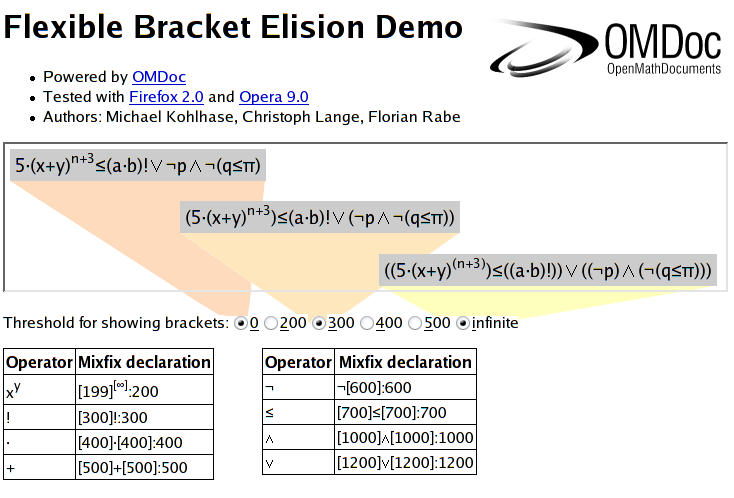
\includegraphics[width=.75\textwidth]{demo-shot}
  \end{center}
\end{frame}

\section[Content Dictionary Format]{The Flexary Mixfix Model in a CD Format}
\label{sec:omdoc2}

\begin{frame}
  \frametitle{An XML Encoding for Flexary Mixfix Declarations}
  Extensions to the declarative {\omdoc} syntax for presentations …
  \begin{itemize}
  \item making it \ExprColor{more expressive}\newline (\ExprColor{flexary
      mixfixes}; embedded XSLT fragments no longer necessary {\large\smiley})
  \item allowing for \ElisColor{flexible elisions}\newline
    (\ElisColor{elision groups} and \ElisColor{visibility levels})
  \end{itemize}
  How is the notation definition for a symbol determined?
  \begin{enumerate}
  \item Look up a presentation for the resp.\ symbol and role.
  \item Otherwise use ``default'' presentation for the home theory.
  \item If there is more than one presentation: choice is non-trivial; see
    [Kohlhase/Müller/Müller] at MathUI.
  \end{enumerate}
\end{frame}

\begin{frame}[fragile]
  \frametitle{Generating Presentations for Content Objects}
  Example: the typing jugdment $\Gamma\vdash_\Sigma t:T$ in {\LaTeX}:
%%% THIS IS JUST AN XML NOTATION FOR THE BOXES WE HAD BEFORE
{\scriptsize
\begin{alltt}
<symbol \textcolor{DarkRed!75}{name="typing-judgment"} \textcolor{violet!75}{role="application"}/>
<presentation \textcolor{DarkRed!75}{for="#typing-judgment"} \textcolor{violet!75}{role="application"} format="latex">
  \textcolor{DarkGreen!75}{<arg pos="1"/>}
  <text>\textcolor{DarkSlateGray!75}{\bsl{}vdash_\{}</text>\textcolor{DarkGoldenrod!75}{<arg pos="2"/>}<text>\textcolor{DarkSlateGray!75}{\}}</text>
  \textcolor{blue!75}{<arg pos="3"/>}
  <text>\textcolor{DarkSlateGray!75}{:}</text>
  \textcolor{DeepPink!75}{<arg pos="4"/>}
</presentation>
\end{alltt}}
  \begin{columns}[T]
    \begin{column}{.5\textwidth}
      \footnotesize Input:
{\scriptsize
\begin{alltt}
\textcolor{violet!75}{<OMA>}
  \textcolor{DarkRed!75}{<OMS name="typing-judgment" cd="typ"/>}
  \textcolor{DarkGreen!75}{<OMS name="emptyset" cd="sets"/>}
  \textcolor{DarkGoldenrod!75}{<OMV name="\(\Sigma\)"/>}
  \textcolor{blue!75}{<OMS name="true" cd="boolean"/>}
  \textcolor{DeepPink!75}{<OMS name="Boolean" cd="boolean"/>}
\textcolor{violet!75}{</OMA>}
\end{alltt}}
    \end{column}
    \begin{column}{.5\textwidth}
      {\footnotesize Output:}
{\scriptsize
\begin{alltt}
\textcolor{DarkGreen!75}{\bsl{}emptyset}\textcolor{DarkSlateGray!75}{\bsl{}vdash_\{}\textcolor{DarkGoldenrod!75}{\(\textcolor{DarkGoldenrod!75}{\Sigma}\)}\textcolor{DarkSlateGray!75}{\}}
  \textcolor{blue!75}{\bsl{}mathit\{true\}}\textcolor{DarkSlateGray!75}{:}\textcolor{DeepPink!75}{\bsl{}mathit\{Boolean\}}
\end{alltt}}
      Rendered: $\textcolor{DarkGreen!75}{\emptyset}\mathop{\textcolor{DarkSlateGray!75}{\vdash}}_{\textcolor{DarkGoldenrod!75}{\Sigma}}\textcolor{blue!75}{\mathit{true}}\mathop{\textcolor{DarkSlateGray!75}{:}}\textcolor{DeepPink!75}{\mathit{Boolean}}$
    \end{column}
  \end{columns}
\end{frame}

\begin{frame}[fragile]
  \frametitle{Generating Presentations for Content Objects}
  Example for flexary notation and multiple output formats:
{\tiny
\begin{alltt}
<symbol \textcolor{DarkRed!75}{name="times"} \textcolor{violet!75}{role="application"}/>
<presentation \textcolor{DarkRed!75}{for="#times"} \textcolor{DeepPink!75}{role="constant"} \textcolor[HTML]{3232B1}{format="ascii"}>
  <text>*</text>
</presentation>
<presentation \textcolor{DarkRed!75}{for="#times"} \textcolor{DeepPink!75}{role="constant"} \textcolor[HTML]{3232B1}{format="latex"}>
  <text>\bsl{}ast</text>
</presentation>
<presentation \textcolor{DarkRed!75}{for="#times"} \textcolor{violet!75}{role="application"}
 precedence="400" \textcolor[HTML]{3232B1}{format="ascii latex"}>
  \textcolor{DarkGoldenrod!75}{<text egroup="lbrack">(</text>}
  \textcolor{DarkGreen!75}{<map begin="1" end="-1">}
    <separator>\textcolor{DeepPink!75}{<arg pos="0"/>}</separator>
    \textcolor{DarkGreen!75}{<recurse precedence="400"/>}
  \textcolor{DarkGreen!75}{</map>}
  \textcolor{DarkGoldenrod!75}{<text egroup="rbrack">)</text>}
</presentation>
\end{alltt}}
  \begin{columns}[T]
    \begin{column}{.5\textwidth}
      {\footnotesize Input:}
{\scriptsize
\begin{alltt}
<apply><power/>
  \textcolor{violet!75}{<apply>}\textcolor{DarkRed!75}{<times/>}
    \textcolor{DarkGreen!75}{<ci>x</ci><ci>y</ci>}
  \textcolor{violet!75}{</apply>}
  <cn>2</cn>
</apply>
\end{alltt}}
    \end{column}
    \begin{column}{.5\textwidth}
      {\footnotesize Output:}
      \begin{description}
      \item[\LaTeX:] $\textcolor{DarkGoldenrod!75}{(}\textcolor{DarkGreen!75}{a}\mathop{\textcolor{blue!75}{\ast}}\textcolor{DarkGreen!75}{b}\textcolor{DarkGoldenrod!75}{)}^2$
      \item[ASCII:] \begin{alltt}\textcolor{DarkGoldenrod!75}{(}\textcolor{DarkGreen!75}{a}\textcolor{blue!75}{*}\textcolor{DarkGreen!75}{b}\textcolor{DarkGoldenrod!75}{)}^2\end{alltt}
      \end{description}
      
    \end{column}
  \end{columns}
\end{frame}

\begin{frame}[fragile]
  \frametitle{Generating Presentations for OpenMath Objects}
  Bracket elision in Presentation {\mathml}:
{\scriptsize
\begin{alltt}
<presentation \textcolor{DarkRed!75}{for="#plus"} precedence="500">...</presentation>
<presentation \textcolor{DarkRed!75}{for="#times"} precedence="400">
  \textcolor{DarkGoldenrod!75}{<element name="mo" egroup="lbrack">
    <text>(</text>
  </element>}
  ...
</presentation>
\end{alltt}}
  \begin{columns}[T]
    \begin{column}{.5\textwidth}
      \footnotesize Input:
\scriptsize
\begin{alltt}
<OMA>
  \textcolor{DarkRed!75}{<OMS name="plus" cd="arith1"/>}
  <OMA>
    \textcolor{DarkRed!75}{<OMS name="times" cd="arith1"/>}
    <OMV name="a"/>
    <OMV name="x"/>
  </OMA>
  <OMV name="y"/>
</OMA>
\end{alltt}
    \end{column}
    \begin{column}{.5\textwidth}
      {\footnotesize Output:}
{\scriptsize
\begin{alltt}
<mrow>
  <mrow>
    \textcolor{DarkGoldenrod!75}{<mo style="display:none"
     omdoc:elevel="100">(</mo>}
    <mi>a</mi>\textcolor{DarkRed!75}{<mo>\(\cdot\)</mo>}<mi>x</mi>
    \textcolor{DarkGoldenrod!75}{<mo style="display:none"
     omdoc:elevel="100">)</mo>}
  </mrow>
  \textcolor{DarkRed!75}{<mo>+</mo>}<mi>y</mi>
</mrow>
\end{alltt}}
    \end{column}
  \end{columns}
\end{frame}

\section{Conclusion and Outlook}
\label{sec:conc}

%%% ALL WE SAID PRESUPPOSES A CONTENT FORMAT; NEED THE FEATURES INTRODUCED HERE
%%% IN A CD FORMAT

\begin{frame}
  \frametitle{Conclusion and Outlook}
  \begin{itemize}
  \item Content-oriented representation formats are independent from a specific
    output format
  \item Human-oriented presentations can be \emph{generated}, w.\,r.\,t.\ user
    preferences, device constraints, \ldots
  \item Need presentation algorithms that are: knowledge-based, extensible,
    adaptive, mathematical, efficient.
    %%% KNOWLEDGE BASED: KNOWLEDGE ABOUT NOTATION
    %%% EXTENSIBLE: MATH IS NEVER FINISHED
    %%% ADAPTIVE: TAKE USER/READER'S PREFERENCES INTO ACCOUNT
    %%% MATHEMATICAL: MODEL AS MANY MATHEMATICAL PRACTICES AS POSSIBLE
    %%% EFFICIENT: PRESENTATION GENERATION IMPLEMENTATION
  \item \ExprColor{Declarative} notation definitions are most manageable.
  \item More general topic: \emph{abbreviation}/\emph{ellipses}
  \item Problem not addressed here: reverse presentation (\emph{parsing})
  \item Prototype implemented, evaluation in progress\newline
    $\leadsto$ {\mathml} 3 recommendation
  \end{itemize}
\end{frame}


\begin{frame}
  \frametitle{References}
  \begin{itemize}
  \item Kohlhase: {\omdoc} -- An open markup format for mathematical documents
    [version 1.2] (2006)
  \item Kohlhase, Müller Ch., Müller N.: Documents with flexible notation
    contexts as interfaces to mathematical knowledge (2007)
  \item Manzoor, Libbrecht, Ullrich, Melis: Authoring Presentation for
    {\openmath} (2005)
  \item Naylor, Watt: Meta style sheets for the conversion of mathematical
    documents into multiple forms (2001)
  \item Paulson: {\isabelle} reference manual (2005)
  \end{itemize}
\end{frame}

%%% BACKUP SLIDES

\begin{frame}[fragile]
  \frametitle{Direct Specification of Symbol Characteristics}
  \begin{itemize}
  \item Syntactical sugar for mixfix notation
    \begin{itemize}
    \item e.\,g.\ right-associative infix: $\imarg{p-1}{1}\to\imarg{p}{2}:p$ 
    \item other pre-defined characteristics: bracket style, pre-/post-/infix
    \item bracket styles for pre-/postfix: mathematical like $f(x)$, or LISP: $(f x)$
    \end{itemize}
  \end{itemize}
  {\scriptsize
\begin{alltt}
<presentation for="\#arrow" format="ascii" role="application">
  <use fixity="infixr">
    <lbrack>(</lbrack>
    <rbrack>)</rbrack>
    <operator><text value=" -\&gt; "/></operator>
  </use>
</presentation>
\end{alltt}}
  \begin{itemize}
  \item Compatible to OMDoc 1.2; {\openmath} standard content dictionaries are supported
    \begin{itemize}
    \item Note: embedded XPath/XSLT no longer necessary and thus no longer
      supported!
    \end{itemize}
  \end{itemize}
\end{frame}

\begin{frame}[fragile]
  \frametitle{A Template-Based Approach to Flexary Mixfix Notations}
  \begin{itemize}
  \item Sometimes, ``deep'' pattern matching \emph{is} more powerful: $\sin^2 x$
  \item Compatible to ActiveMath -- not syntactically but conceptually
  \item Re-use most of the syntax of the symbol-pased approach
  \item Same syntax for input and output specification $\Rightarrow$ both
    presenting content and parsing presentation to content supported {\large \smiley}
  \end{itemize}
  \begin{columns}[T]
    \begin{column}{.5\textwidth}
      {\tiny
\begin{alltt}
<presentation \textcolor[HTML]{3232B1}{format="OM"} \textcolor{DarkRed!75}{for="#typing-judgment"}>
  <OMA><OMS cd="types" \textcolor{DarkRed!75}{name="typing-judgment"}/>
    \textcolor{DarkGoldenrod!75}{<arg name="context"/>}
    \textcolor{DarkGreen!75}{<arg name="sig"/>}
    \textcolor{DeepPink!75}{<arg name="term"/>}
    \textcolor{violet!75}{<arg name="type"/>}
  </OMA>
</presentation>
\end{alltt}}
        (Note: literally included \texttt{<element>} constructors!)
      \end{column}
      \begin{column}{.5\textwidth}
      {\tiny
\begin{alltt}
<presentation \textcolor[HTML]{3232B1}{format="pmathml"} \textcolor{DarkRed!75}{for="#typing-judgment"}>
  <mrow>
    \textcolor{DarkGoldenrod!75}{<arg name="context"/>}
    <msub><mo>\(\vdash\)</mo>\textcolor{DarkGreen!75}{<arg name="sig"/>}</msub>
    \textcolor{DeepPink!75}{<arg name="term"/>}
    <mo>:</mo>
    \textcolor{violet!75}{<arg name="type"/>}
  </mrow>
</presentation>
\end{alltt}}
      \end{column}
    \end{columns}
\end{frame}

\end{document}
